\documentclass[12pt]{article}
\usepackage{enumitem}
\usepackage{mathtools}
\usepackage{amsthm}
\usepackage{graphicx}
\graphicspath{ {images/} }
\begin{document}

\title{Assignment 5}
\author{Darwin Ding}
\maketitle

\section*{Exercise 2.8}
\begin{enumerate}[label=(\alph*)]
	\item By definition, $\bar{g}$ is a linear sum of all of the picked hypotheses in H multiplied by a constant factor. Since the learning algorithm will always pick a hypothesis from H for each g, and because H is closed under linear combination, $\bar{g}$ is in H.
	\item A very simple example can be found in binary classification, if H contains just the hypothesis that returns +1 for all x and the hypothesis that returns -1 for all x. Let's say we're going to generate a random data set of points that are either +1 or -1 with equal probability, and the learning algorithm is going to pick the hypothesis that agrees with the data set the most.
	\\ \\ Clearly, both hypotheses will be picked with equal probability. Therefore, the average function, $\bar{g}$, would return 0 for all x and is clearly not present in this set.
	\item No, not at all. With a complex number of hypotheses, you should expect the average to be very fractional in nature. For instance, if there were 10 final hypotheses that return +1 for a data point and 5 that return -1 for that data point, $\bar{g}$ should return +0.5, which is clearly not a binary output.
\end{enumerate}

\section*{Problem 2.14}
\begin{enumerate}[label=(\alph*)]
	\item Suppose that $d_{VC} = n$ for all hypothesis sets from $H_1$ to $H_K$. This means that for each of these sets, there is a set of $n$ points that can be completely shattered by that hypothesis set. When merging two of these hypothesis sets, the $d_{VC}$ will double as long as there exists a non-overlapping set of size $n$ from each set that can be shattered by the hypothesis sets separately. If this is not the case, the final $d_{VC}$ of the union will be $d_{VC}*2 - overlap$, where overlap is the minimum number of points shared by the two picked sets.
	\\ \\ Following from this, it is clear that when adding up all K sets, the maximum $d_{VC}(H)$ is $Kn$. This is also the best case scenario, where we can find K non-overlapping sets of n points that can independently be shattered by each of the hypothesis sets. If there is overlap, $d_{VC}(H) < Kn$.
	\\ \\ Since $K(d_{VC} + 1) > K(d_{VC}) = Kn$, this inequality is true.
	\item Each of the individual hypothesis sets, $H_1$ thru $H_K$, can implement (on sets of $l$ points) at most $l^n + 1$ dichotomies (using $d_{VC} = n$ as before). If each hypothesis set can implement $l^n + 1$ dichotomies, then at most, K hypothesis sets can implement $Kl^n + K$ dichotomies on sets of l points (of course the actual number being bounded by $2^l$). (This generous bound also assumes that each of the K hypothesis sets are providing $l^n+1$ unique dichotomies to this total).
	\\ \\ However, we are given $2^l > 2Kl^n$, and $2Kl^n \ge Kl^n + K$ (they are equal when $n = 0$, which happens if the hypothesis set cannot even shatter 1 point). Naturally, $\boldsymbol{2^l > Kl^n + K \ge m_H(l)}$.
	\\ \\ $2^l > m_H(l)$ occurs only when $d_{VC}(H) < l$. This is because for all points N where $N \le d_{VC}(H)$, $m_H(N) = 2^N$. Therefore, $d_{VC}(H) \le l$.
	\item From part a, we know that $d_{VC}(H) \le K(d_{VC} + 1)$.
	\\ \\ We've also shown that $d_{VC}(H) \le l$, so essentially we bound by the minimum of $l$ and $K(d_{VC} + 1)$. Let's assume $l$ takes on the value shown, we just need to verify that it satisfies the bound presented in b.
	\begin{gather*}
	2^l > 2Kl^n
	\\ 2^{7(n + K)log_2{nK}} > 2K(7(n+K)log_2{nK})^n
	\\ 2^{log_2{(nK)^{7(n + K)}}} > 2K7^n(n+K)^n(log_2{nK})^n
	\\ (nK)^{7n + 7K} > 2K7^n(n+K)^n(log_2{nK})^n
	\end{gather*}
	In this problem, n is a constant that is true for all hypothesis sets. As a result, the right hand side is a polynomial expression that will grow somewhat quickly as K, a non-constant factor, increases. However, on the left hand side, there is a K in the exponent, which means it grows at a crazy exponential rate. As a result, the inequality holds, and $m_H(x)$ is bounded by the minimum of $l$ and the expression from part a.
\end{enumerate}

\section*{Problem 2.15}
\begin{enumerate}[label=(\alph*)]
	\item One example of a monotonic classifier in two dimensions is $h(x, y) = sign(x + y)$ (with $x + y = 0$ returning $+1$), where x and y are the dimensions of each incoming point. This is monotonic because for any two points ($x_0$, $y_0$), ($x_1$, $y_1$), if $x_0 \ge x_1$ and $y_0 \ge y_1$, then $sign(x_0 + y_0) \ge sign(x_1 + y_1)$.
	\item Note that if you follow the hint and start with a single point, then push one dimension up and another down continuously to generate the rest of the points, none of the points (through the definition given in the problem) are ever considered larger than any of the others.
	\\ \\ As a result, it doesn't matter what any of the points are or how many there are, all dichotomies can be implemented by one of the infinitely many monotonically increasing functions. This is due to the fact that there are no restrictions on monotonically increasing function behavior on "equal" points.
	\\ \\ Therefore, the VC dimension is $\boldsymbol{\infty}$, because the growth function $m_H(N) = \boldsymbol{2^N}$ for all N.
\end{enumerate}

\section*{Problem 2.24}
\begin{enumerate}[label=(\alph*)]
	\item The average function is essentially the expected value of the output function based off of the two points.
	\\ \\ If we pick two arbitrary points ($x_0$, $x_0^2$), ($x_1$, $x_1^2$), the slope we generate will be $(x_1^2 - x_0^2)/(x_1 - x_0) = x_0 + x_1$. Since the expected value of both $x_0$ and $x_1$ are 0, the expected value of the slope will be $0$. This makes sense, because the slope of the $x^2$ function is $2x$, and so we are basically giving the slope at $x = 0$, at the middle of the interval.
	\\ \\ In the equation: $y = mx + b$, we can plug in either data point to determine b now that we have the expected slope: $x^2 = x + b$. Since the expected value of x here is 0, we can solve for b: $0 = 0 + b \implies b = 0$.
	\\ \\ Thus, our $\bar{g}$ is $\boldsymbol{y = 0}$.
	\item We can generate thousands of sample data sets within the interval and then calculate the final hypothesis g based off of each data set. From then, we can average all of the lines created to create $\bar{g}$. Using $\bar{g}$ we can calculate the bias by running $\bar{g}$ against our $f(x) = x^2$ inside the interval. For variance, we can also run each of our test lines against $\bar{g}$ and average that.
	\item Results after running on 1000 test data sets: 
	\\ 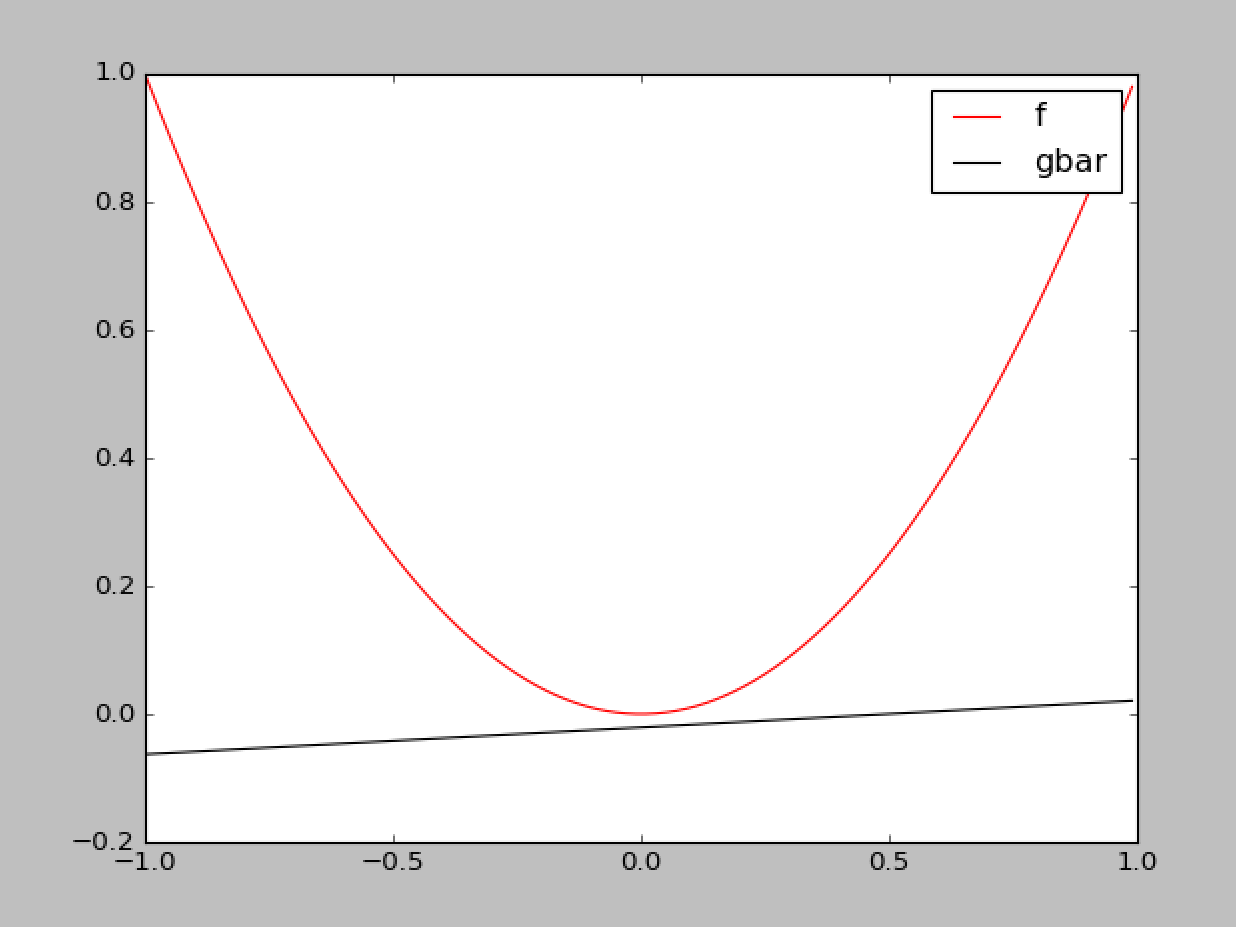
\includegraphics[scale=.5]{2-24.png}
	\\ $\bar{g} = 0.042x-0.021$
	\\ $E_{out} = 0.54416$
	\\ $bias = 0.2150$
	\\ $variance = 0.32916$
	\item We can calculate $bias$ by taking the integral of $(f - 0)^2$ over the interval and dividing by the size of the interval. This is basically plugging the values into the bias formula and making the step size continuous versus discrete.
	\begin{gather*}
	bias = 0.5 \int_{-1}^{1}x^4 dx = 0.5(0.4) = \boldsymbol{0.2}
	\end{gather*}
	For variance we can approach this similarly to before, by adapting the variance formula into a continuous calculation. Note that below, $\bar{g} = 0$. Once we simplify the formula, we take the integral over the formula and divide by the size of the integral to get the expected value.
	\begin{gather*}
	var(x) = E[(g^{(D)}(x) - \bar{g}(x))^2]
	\\ = E[g^{(D)}(x)^2 - 2g^{(D)}(x)\bar{g}(x) + \bar{g}(x)^2]
	\\ = E[g^{(D)}(x)^2]
	\\ = 0.5 \int_{-1}^{1}x^2 = \boldsymbol{0.333}
	\end{gather*}
	$E[E_{out}] = bias + var = 0.2 + 0.333 = \boldsymbol{0.533}$
\end{enumerate}
\end{document}